\documentclass{standalone}
\pagestyle{empty}
\usepackage{tikz}
\usetikzlibrary{arrows.meta,bending}

\begin{document}
\noindent
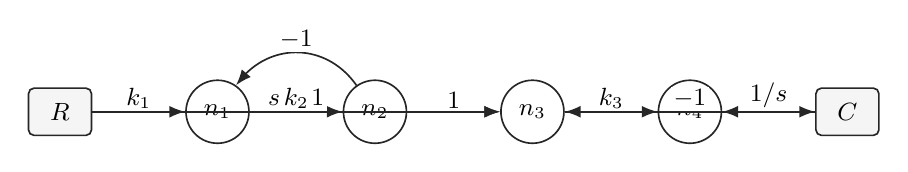
\begin{tikzpicture}[
  >=Latex,
  ->,
  semithick,
  every node/.style={font=\small},
  signal node/.style={circle,draw,minimum size=8mm,inner sep=1pt,fill=white},
  io node/.style={rectangle,rounded corners=2pt,draw,minimum width=8mm,minimum height=6mm,inner sep=2pt,fill=gray!8},
  every path/.style={draw=black!85},
  edge label/.style={fill=white,inner sep=1pt,text=black},
]
\node[signal node] (n1) at (2.0,3.0) {$n_1$};
\node[signal node] (n2) at (4.0,3.0) {$n_2$};
\node[signal node] (n3) at (6.0,3.0) {$n_3$};
\node[signal node] (n4) at (8.0,3.0) {$n_4$};
\node[io node] (R) at (0.0,3.0) {$R$};
\node[io node] (C) at (10.0,3.0) {$C$};
\draw (R) -- node[edge label,midway,above] {$k_1$} (n1);
\draw (n2) to[out=125,in=55,looseness=1.14] node[edge label,midway,above] {$-1$} (n1);
\draw (n1) -- node[edge label,midway,above] {$s+1$} (n2);
\draw (n2) -- node[edge label,midway,above] {$1$} (n3);
\draw (R) -- node[edge label,midway,above] {$k_2$} (n3);
\draw (C) -- node[edge label,midway,above] {$-1$} (n3);
\draw (n3) -- node[edge label,midway,above] {$k_3$} (n4);
\draw (C) -- node[edge label,midway,above] {$-1$} (n4);
\draw (n4) -- node[edge label,midway,above] {$1/s$} (C);
\end{tikzpicture}
\end{document}
